\chapter{Proposed Gait Recognition System} \label{ch:methodology}
In this chapter, we are going to discuss the proposed framework and its main components in detail. In Section~\ref{sec:preprocess}, we will explain the data collection and preprocessing steps. In Section~\ref{sec:extract_feature_vector} and Section~\ref{sec:feature_preprocess}, the proposed spatio-temporal gait feature extraction and preprocessing techniques are elaborated respectively in detail. The network architectures of our proposed algorithm for both single-view and multi-view gait recognition are illustrated in Section~\ref{sec:single_view_arch} and Section~\ref{sec:multi_view_arch} respectively. 



%------------------------------------------------------------------------------------------
\section{Data Preprocessing} \label{sec:preprocess}
From 2D pose estimation algorithm~\cite{Cao_19}, we got raw 2D coordinates for each body joint, as shown in Figure~\ref{fig:pose_estimation}. In this work, several preprocessing steps have been undertaken to build a compact, robust and discriminative descriptor based on these raw coordinates. In this section, we are going to discuss these steps in detail.

\subsection{Collecting Pose Information}
Let $D = {\{{v_{i},s_{i}\}}^{N}_{i=1}}$ be the gait dataset containing $N$ samples. $v_i$ represents the ${i}^{th}$ subject's RGB gait video. $s_{i} \epsilon L$ represents the ${i}^{th}$ subject ID, where $L$ is the set of target IDs.  Let $\mathcal{T} \subset \mathcal{D}$ be the chosen training subset and $\mathcal{T^\star} = \mathcal{D} \setminus \mathcal{T}$ the testing subset. From the OpenPose algorithm~\cite{Cao_19} we get a mapping between the RGB data and the body skeleton as:

\begin{equation}
v_i^{(t)}\quad \xrightarrow[]{\text{pose detector}}\quad \mathbf{p}_i^{(t)} \qquad\forall t= 1,...,T_i 
\end{equation}

where, $\mathbf{p}_i^{(t)}$ represents the ${i}^{th}$ sample pose at frame $ t $ and $T_i$ represents the time-length of sample $i$. In particular, $\mathbf{p}_i^{(t)}$ consists of a list of 2D coordinates:

\begin{equation}
\mathbf{p}_{i}^{(t)} ={(x_j^{(t)}, y_j^{(t)})_{i}} \qquad j~\epsilon~J
\end{equation}
where $j$ represents the joint index and $J$ is the joints set defined by the pose estimation algorithm. Thereafter, we exploit these RGB-poses mapping provided by the Openpose algorithm to design a novel 50-D spatio-temporal feature vector for each frame and transformed them into a time series to train a RNN network.


\begin{figure}
	\centering 
	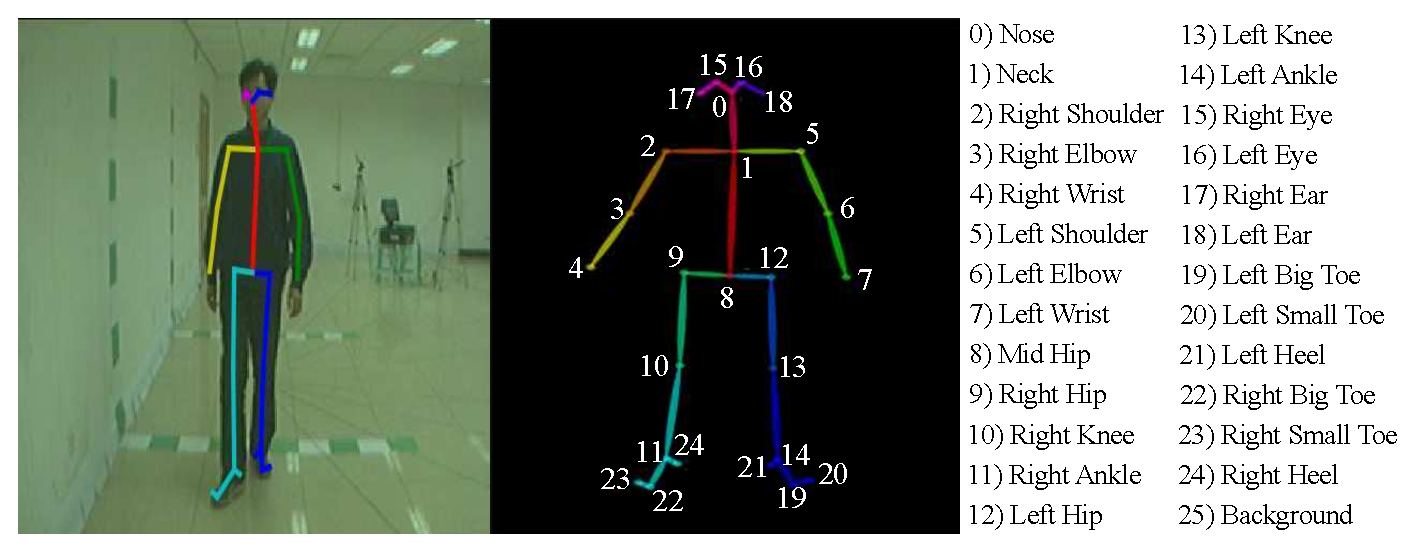
\includegraphics[width = \textwidth]{figures/pose_estimation.eps}
	\caption[Examples of 2D human pose estimation from RGB images of CASIA dataset]
	{Examples of 2D human pose estimation by~\cite{Cao_19} from RGB images of CASIA dataset. \label{fig:pose_estimation}}
\end{figure}


\subsection{Handling Missing Joint Information}
One of the most challenging tasks for the pose estimation algorithm to estimate the pose of a subject who is completely or partially occluded. This scenario often leads the algorithm to fail in estimating one or more joint coordinates. In order to make our proposed gait algorithm robust and accurate, we have to address the problem of missing joint information carefully. So, it is of vital importance to make an algorithm that can estimate the whole body joints set appropriately. In this thesis, we employed the following strategies which are proven to be effective in addressing the missing joint problem:

\begin{itemize}
	\item The center of the hip joint is considered as the origin of the coordinate system. Now, any frame is rejected where the origin can not be located due to the missing hip joints;
	\item If more than one body joints are missing in between the knee and the hip joints of both leg, the frame is rejected;
	\item Persistent missing joints are calculated by exploiting the left and right side body symmetry;
	\item In other cases, a position of $[0.0, 0.0]$ is given to the joint which was not located in the frame.
\end{itemize}

The above strategies are simpler and do not require any computation. They are also proven to be effective in addressing the missing data problem. Algorithm~\ref{alg:missing_data} depicts the proposed techniques for handling missing joint information.

\begin{algorithm}
	\caption{Algorithm for Handling Missing Joints Information}
	\label{alg:missing_data}
	\begin{algorithmic}
		\input{algorithms/missing_data.alg}
	\end{algorithmic}
\end{algorithm}


\subsection{Normalization}
It is very important to normalize the skeletal data with regard to the subject position in the frame. Since in most of the gait videos people walk through the fixed camera, the size of the subject's skeleton changes due to the variation of the distance between the subject and the camera. Therefore, we have to normalize the gait sequence, i.e., keeping the subject size and the camera to subject distance constant for improved performance. Therefore,  in order to eliminate different sizes and location variations of the human skeleton we had to transform the 2D  coordinates of all joints into a new coordinate system whose origin can be the middle of the hip ($\mathbf{J}_{o}$). To find the origin of the coordinate system ($\mathbf{J}_{o}$) for each subject, in this research, we considered the right, left, and middle of the hip joints and calculated the average of them. 

\begin{equation} 
\begin{split}
\mathbf{J}_{o} = {(x̄_{o} , y_{o})} &= {(\mathbf{J}_{LHip} +\mathbf{J}_{RHip} +\mathbf{J}_{MHip})} / {3} \\
(\bar{x}̄_{i} , \bar{y}_{i}) & = {(x̄_{i} , y_{i})} - {(x̄_{o} , y_{o})}~~~~\forall j \epsilon \mathbf{J}
\end{split}
\end{equation}
Here, $(\bar{x}̄_{j} , \bar{y}_{j})$ is set by root-centered coordinate reference system defined by above equations. Again, we normalized the skeletons of different subjects to fixed size by considering $ h $, the Euclidean distance from hip to neck joint, as unit length. The following equation shows the normalization procedure of the raw 2D joints:


\begin{equation} \label{equ:normalization_raw_joint}
\begin{split}
h &= \parallel \mathbf{J}_{o} - \mathbf{J}_{neck} \parallel_2  \\
\mathbf{J}_{i}^{N} &= (\bar{\bar{x}̄}_{i} , \bar{\bar{y}}_{i}) = (\bar{x}̄_{i} , \bar{y}_{i}) / h 
\end{split}
\end{equation}
Here, $\mathbf{J}_{i}^N$ be the new coordinate of the $i^{th}$ joint $\mathbf{J}_{i}$ of a particular pose. These two steps of normalization have huge impact on the robustness of the gait recognition algorithm. Firstly, they allow fair comparisons between different subject's poses reducing the effect due to variation of subject size and position in the camera. Secondly, as it discards the absolute coordinates of subject's body pose, pose size become homogeneous among different camera settings and proximity to camera. Thus, it makes the system robust to zooming, camera position, and subject location. 




%-------------------------------------------------------------------------
\section{Extracting Spatio-Temporal Feature Vector} \label{sec:extract_feature_vector}
The workflow of the proposed network is illustrated in Figure~\ref{fig:overview_proposed_method}. Many strategies have been taken to design a lower-dimensional spatio-temporal feature descriptor based on the 2D human poses estimated from the raw video frames. In this section, we elaborate on the feature extraction procedure of our proposed method. 

\begin{figure}
	\centering
	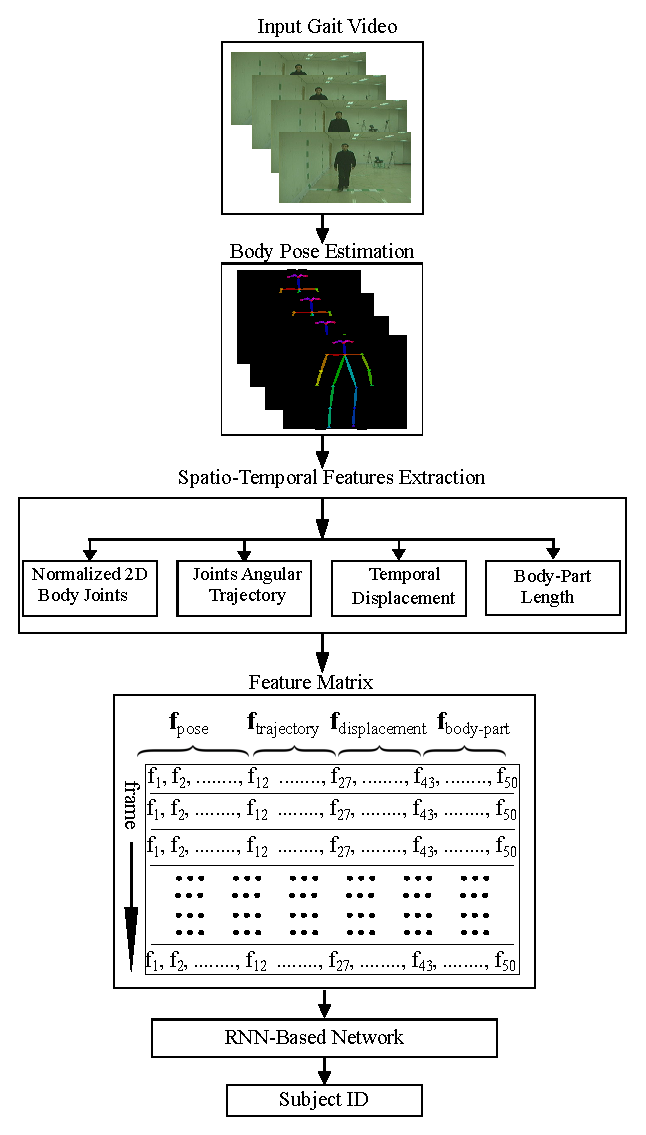
\includegraphics[width=0.8\textwidth]{figures/proposed_method.eps}
	\caption [The overview of the proposed framework for gait recognition] 
	{The overview of the proposed framework for gait recognition.  \label{fig:overview_proposed_method}
	}	
\end{figure}

\subsection{2D Body Joint Features}
As all the joints of the human body do not play a significant role in gait pattern, they cannot improve gait recognition accuracy. Some joints perform even worse. So, among the 25 body joints estimated from the OpenPose algorithm, we searched out for those joints which have a rich and discriminative gait representation capacity. Cunado \textit{et al.}~\cite{Cunado_97} used the human leg-based model as they found that the change of human leg contains the most important features for gait recognition.  In our study, we found that the knee along with the joints located in the feet shows more robustness than any other body joints because they do not alter while people are walking in clothes or carrying bags. Some joints, e.g. hip, get wider in coat than normal condition. Again, in some gait videos, some subjects put their hands into their coat pocket, which they cannot do in normal walking. This situation significantly changes the joint coordinates. Therefore, raw body joints above the hip do not have any significant impact on gait pattern. Hence, in our method, we did not consider the hip or any other body joints above it.



\begin{figure}
	\centering 
	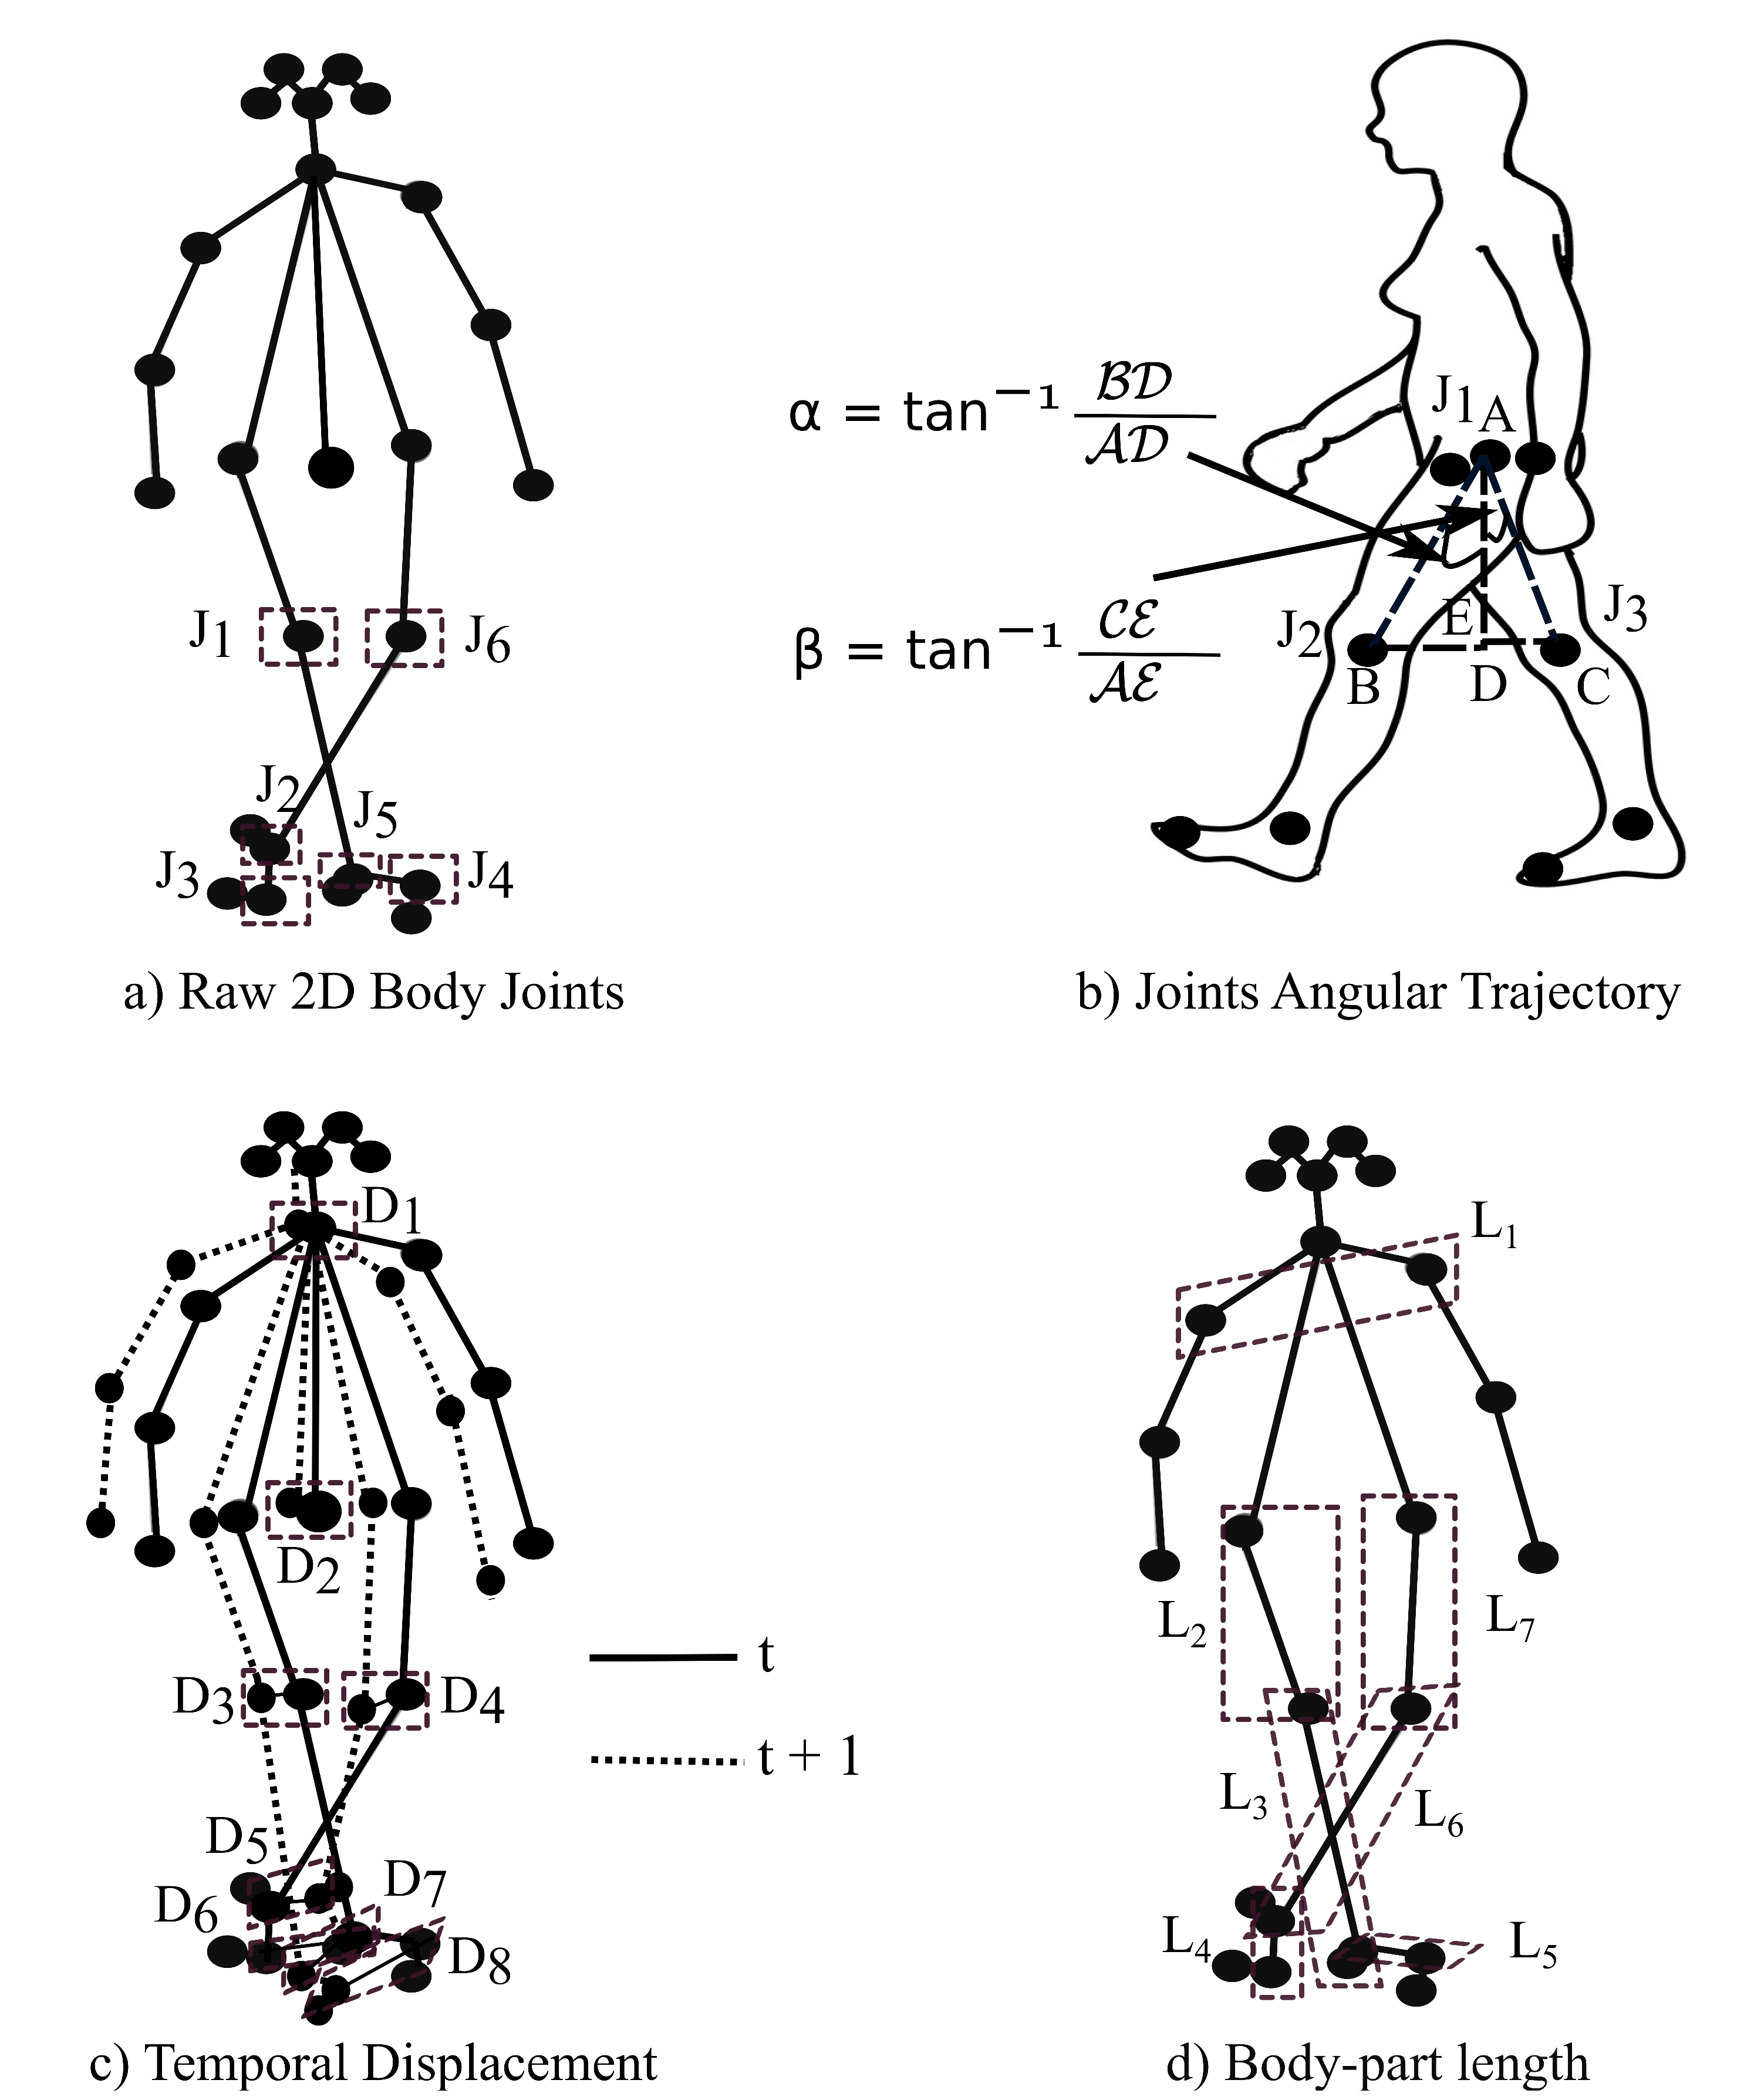
\includegraphics[width = 0.7\textwidth]{figures/extracted_features.eps}
	\caption[Scheme for the four different types of feature extraction process of the proposed method]
	{Scheme for the four different types of feature extraction process of the proposed method. a) 6 effective joints were selected out of 25 body joints. b) 5 angular trajectories from the lower limbs were considered to form a joint-angle feature vector. c) A total of 8 body joints were selected to get a temporal displacement feature vector. d) 7 body parts were taken to form a body part length feature vector.\label{fig:extracted_features}
	}
\end{figure}

Consequently, in our work, as shown in Figure~\ref{fig:extracted_features}a, we selected 6 body joints (RKnee, Rankle, RBigToe, LKnee, LAnkle, LBigToe) to form the effective body pose features. Thus, we have 12-D pose feature vector, $\textbf{f}_{body-joint}$, for a single frame. 

\begin{equation}
  \textbf {f}_{body-joint}= [x_1, y_1, x_2, y_2, \ldots\ldots, x_6, y_6]^T
\end{equation}




\subsection{Joint Angular Trajectory}
The dynamics of gait motion can be expressed by the temporal information of joint angles. Therefore, discriminative gait features can be found by considering the change in joint-angle trajectories of the lower limbs~\cite{Wang_04}. So, in this study, we formulated another 15-dimensional feature vector $\boldsymbol{f}_{trajectory}$ by considering five lower limb joint-angle trajectories using the following equations: 

\begin{table}
	\centering
	\caption{List of selected joint-angle trajectories with corresponding body joints set in order to form a joint angular feature vector. \label{table:list_joint_angle_trajectory}}
	\begin{tabular}{cc}
		\hline
		\textbf{Angular Trajectory} & \textbf{Body Joints Set}\\
		
		\hline
		Hip trajectory &10, 8, 13 \\
		Right knee trajectory  &11, 10, 9 \\
		Left knee trajectory &14, 13, 12 \\
		Right ankle trajectory &22, 11, 10 \\
		Left ankle trajectory &19, 14, 13 \\
		\hline
	\end{tabular}
\end{table}

\begin{equation}
	\begin{split}
	\alpha &= 
	\begin{cases}
	\tan^{-1}{\frac{|J_{2,x}-J_{1,x}|}{|J_{2,y}-J_{1,y}|}} & J_{2,y} \neq J_{1,y}\\
	\pi/2 & J_{2,y} = J_{1,y}
	\end{cases} \\ \noalign{\vskip10pt}
	\beta &= 
	\begin{cases}
	\tan^{-1}{\frac{|J_{3,x}-J_{1,x}|}{|J_{3,y}-J_{1,y}|}} & J_{3,y} \neq J_{1,y}\\
	\pi/2 & J_{3,y} = J_{1,y}
	\end{cases} \\ \noalign{\vskip10pt}
	\theta &= \alpha + \beta
	\end{split}
\end{equation}

As shown in Figure~\ref{fig:extracted_features}b, $J_1, J_2, J_3$ are the joints which form a set of angular trajectory. In this work, we considered total five sets of angular trajectories from the lower limb of human body. Table~\ref{table:list_joint_angle_trajectory} demonstrated the selected angular trajectories with their corresponding body joints. For each trajectory, we took $(\theta, \alpha, \beta)$ as gait features. 

\begin{equation}
\textbf {f}_{trajectory}= [\theta_1, \alpha_1, \beta_1,\theta_2, \alpha_2, \beta_2,\ldots\ldots, \theta_5, \alpha_5, \beta_5]^T
\end{equation}


\subsection{Temporal Displacement}
Our third type of feature extractor is a simple descriptor that preserves temporal information of the gait pattern. It basically stores the local motion features of gait by keeping the displacement information between the two adjacent frames of the subject's pose sequence. The displacement of each coordinate of a joint was then normalized by the total length of displacement of all joints. Let, $t$, and $(t + 1)$ are two adjacent frames of a particular pose sequence. Now, the displacement information of the coordinates of any joint of frame $t$ would be the normalized difference between the corresponding coordinates of two adjacent frames. 

\begin{equation}
\begin{split}
\triangle x^{t}_{1} &=\frac{x^{t+1}_{1} - x^{t}_{1}}{\sum_{i=1}^{8}\parallel J^{t+1}_{i,x} - J^{t}_{i,x}\parallel_2} \\ 
\triangle y^{t}_{1} &=\frac{y^{t+1}_{1} - y^{t}_{1}}{\sum_{i=1}^{8}\parallel J^{t+1}_{i,y} - J^{t}_{i,y}\parallel_2} \\ 
{\bf f}_{displacement} &= [\triangle x_{1}, \triangle y_{1}, \triangle x_{2}, \triangle y_{2} \ldots\ldots, \triangle x_{8}, \triangle y_{8}]^{T}
\end{split}
\end{equation}

Here, $J_i^{t}$ is the 2D coordinates of the $i^{th}$ body joint at $t^{th}$ frame in the video and $(\triangle x_1^t , \triangle y_1^t )$ is the displacement of the coordinates of first joint at $t^{th}$ frame of the video. As shown in Figure~\ref{fig:extracted_features}c, we selected 8 joints (Neck, MHip, RKnee, Rankle, RBigToe, LKnee, LAnkle, LBigToe) to get a 16-dimensional feature vector, $\textbf{f}_{displacement}$.


\subsection{Body Part Length Features}
The static gait parameters, for example, the length of the body parts calculated from the raw body joints position are also very important for gait recognition~\cite{Wang_04, Araujo_13}. They form a spatial gait feature vector which makes them robust against covariate factors such as carrying and clothing condition variation. In this study, we took a total of seven body parts (Figure~\ref{fig:extracted_features} (d)) namely length of the two leg, two feet, two thighs, and width of the shoulder which formed a 7-dimensional spatial feature vector $\textbf{f}_{body-part}$. 


\subsection{Fusion of Features}
A lot of research works have been done to fuse multiple features to get improved performance~\cite{Liao_19, Wang_04}.  Different types of fusion methods were proposed in literature such as feature level fusion, representation level fusion, and score level fusion. In feature level fusion, multiple features of the same frame are concatenated before feeding into a final network, and in representation level fusion, each feature vector is firstly fed into a network and the resulting global representations are then concatenated to train a final classifier. For a score level fusion, each feature vector is separately fed into the final network which predicts a classification score. Then, the scores from multiple classifiers are fused using an arithmetic mean.

In this study, we found that feature level fusion has produced better recognition results in contrast to other fusion techniques or individual feature sets. 




%------------------------------------------------------------------------------------------
\section{Feature Preprocessing} \label{sec:feature_preprocess}
In this section, we are going to discuss the preprocessing steps that are employed on the proposed feature vector before feeding into the main RNN network.

\subsection{Feature Map}
In this work, we designed a 50-dimensional spatio-temporal gait feature vector \textbf{f} from the raw 2D pose estimation of each frame.  Firstly, we split a gait video into 28 frame segments. Each $28$ frame-segment formed a timestep which can be described by the following equations. 

\begin{equation}
\label{equ:feature_preprocess}
\begin{split}
\boldsymbol{f} &= {[f_1, f_2, f_3, \ldots \ldots, f_{50}]}^T \\
\boldsymbol {T} &= {[\boldsymbol f_1, \boldsymbol f_2, \boldsymbol f_3,  \ldots \ldots, \boldsymbol f_{28}]}^T \epsilon \quad \mathbb {R}^{28\times 50}\\
\boldsymbol V &= {[\boldsymbol T_1, \boldsymbol T_2, \boldsymbol T_3,  \ldots \ldots \boldsymbol T_{N}]}^T 
\end{split}
\end{equation}

Here, \textbf{f} is the 50-dimensional pose vector for each frame; \textit{\textbf{T}} is the feature matrix for each timestep; $ N $ is the total number of timestep sequence, and \textit{\textbf{V}} is the sequence of features for a gait video. 



\subsection{Data Augmentation}
The performance of deep neural networks is strongly correlated with the amount of available training data. Although, CASIA~\cite{Yu_06} is the largest gait dataset, the standard experimental setup of this dataset (see Table ~\ref{table:caisab_setup}) allows us to train on with only the four normal walking sequences for each subject. Hence, we need to augment our train data to obtain a stable model. One way to increase the amount of training data is to overlap video clips. So, we split the input video into an overlapping sequences of video clips. For every 28 image clip, we overlapped 24 images of the previous clip at almost $ \textbf{85.7\%} $ overlapping rate. For example, a particular gait video of 100 frames would be split into the clips $(1-28), (5-32), (9-36), ...$ up to frames $(73, 100)$. 

Again, in the CASIA dataset, gait videos of different subjects have varying timesteps. The number of timesteps in each gait video depends on the total number of frames where a subject is detected. Due to the position of the camera, some angles ${(0^{\circ}, 18^{\circ}, 36^{\circ})}$ have more subject detected frame than other angles ${(72^{\circ}, 90^{\circ}, 108^{\circ})}$. Therefore, the total number of timesteps in a gait video is different for different subjects and view angles. This varying timestep makes our train dataset unbalanced. Again, in the CASIA B dataset, every subject has not had all the gait videos; there are some missing gait videos. To solve the problem and to improve the performance we have to develop our own balance training set by making each subject pose sequence to have a fixed number of timesteps. We first found the subject which had maximum timesteps for a particular gait angle and then augmented other subject's timesteps with that specific length by overlapping their sequences.

In addition to above technique, we further augment our training data by adding another gait sequence (i.e., $ 25\% $ increment) by implementing Gaussian noise to a given normal walking sequence. 

\begin{equation}
N(j_i) = (x + \tilde{x},  \quad y+ \tilde{y})
\end{equation}

Here,  $\tilde{x}$ and $\tilde{y}$ are two random real numbers generated by a normal distribution with zero mean and unit standard deviation. We apply noising ($ N $) into the raw joints position of a training pose data.



%-------------------------------------------------------------------------
\section{Single-View Gait Recognition} \label{sec:single_view_arch}
In this section, we will present the details of the architecture and training procedure of our proposed network for single-view gait recognition. We will also try to describe why our proposed 2-layer BiGRU network is best in modeling the gait descriptors for recognizing the subject ID.

\subsection{Network Architecture}
\begin{figure}
	\centering 
	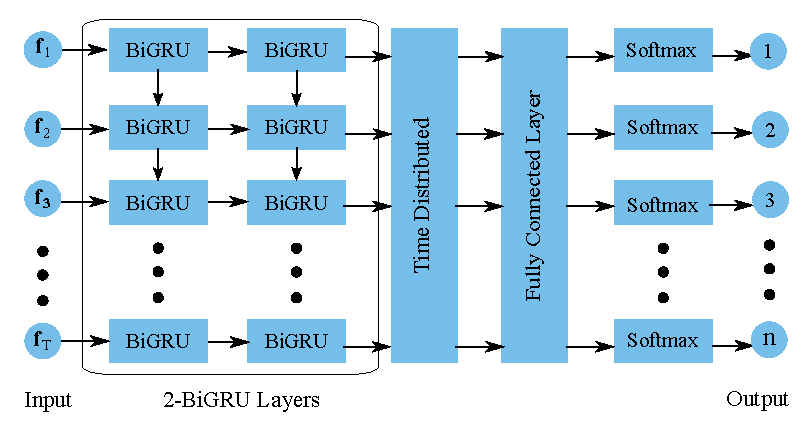
\includegraphics[width = .94\textwidth]{figures/rnn_network.eps}
	
	\caption[Proposed architecture of the temporal network for subject identificatio]
	{Proposed architecture of the temporal network for subject identification.  \label{fig:rnn_network}}
\end{figure}


In this research, we experimented with different \gls{rnn} architectures such as gated recurrent units (\gls{gru}s),  long short-term memory units (\gls{lstm}s), bidirectional long short-term memory (\gls{bilstm})~\cite{Graves_05} and bidirectional gated recurrent units (\gls{bigru})~\cite{Schuster_97}. Firstly, we designed the proposed network employing all these architectures with one recurrent layer and then searched for optimum recurrent unit size between 50 to 100. Henceforth, we increased the capacity of the network by adding the second and third layers of hidden units. Finally, we found that, among different RNN architectures, 2-layer \gls{bigru} performs best. Again, we chose \gls{gru} in our proposed network architecture as it achieves high performance and requires a reduced number of parameters while still retaining long-term temporal information. Now, from the extensive experimental evaluation, as described in Section~$5.2.3$, the optimal size of the latent space representation of our proposed autoencoder was found to be 80.

After the input and the second recurrent layer, we placed a batch normalization (\gls{bn})~\cite{Ioffe_15} layer. At last, a fully connected layer with softmax activation was used to predict the subject classes. Figure~\ref{fig:rnn_network} illustrates the architecture of the proposed network. 


\subsection{Loss Function}
In this work, we found that due to the influence of various covariate factors, intraclass distance related to one subject is sometime more significant than interclass distance. So, if we only use the \textit{cross-entropy loss} as our objective function, the resulting learned features may contain large intraclass variations. Therefore, to effectively reduce the intraclass variations, we employed \textit{center loss} as introduced by Wen \textit{et al.}~\cite{Wen_16} for face recognition task. 

Now, as the training progresses, the center loss learns a center for the features of each class. Also, the distances between the features and their corresponding class centers are minimized simultaneously. However, using only center loss may lead the learned features and the centers close to zeros due to the very small value of the center loss. Hence, with the fusion of softmax loss ($L_s$) and center loss ($L_c$), we can achieve discriminative feature learning by increasing interclass dispersion and compacting intraclass distance as much as possible.


\begin{equation} \label{equ:loss_functions}
\begin{split}
L_s &=-\sum_{i=1}^{m}log{\frac{e^{W_{y_i}^{T}x_i + b_{y_i}}}{\sum_{j=1}^{n}{e^{W_{j}^{T}x_i+ b_j}}}} \\
L_c &= \frac{1}{2}\sum_{i=1}^{m}{\parallel{{\boldsymbol x_i}-{\boldsymbol c_{y_i}}}\parallel}_2^2 \\
L &= L_s + \lambda L_c + \lambda_{\theta}\parallel{\theta}\parallel_{2}
\end{split} 
\end{equation}

Equations~(\ref{equ:loss_functions}) describe the total loss ($ L $) calculation of our proposed network. Here, $\boldsymbol x_{i}~\epsilon~\mathbb {R}^d$ denotes the $i^{th}$ pose sequence which belongs to the $y_i^{th}$ class and  $\boldsymbol c_{y_i}~\epsilon~\mathbb {R}^d$ denotes to the $y_i^{th}$ class center of the learned pose features. $W~\epsilon~\mathbb {R}^{d\times n}$ is the feature dimension of the last fully connected layer and $b~\epsilon~\mathbb {R}$ is the bias term of the network. The batch size and the class number are $ m $ and $ n $ respectively. $\lambda$, a scalar variable, is set to value $ 0.01 $ to balance between the two loss functions. $\parallel{\theta}\parallel_{2}$ refers to the kernel regularizer for all the parameters of the network with a weight decay coefficient $(\lambda_{\theta})$ set to $0.0005$ for the experiment.  


\subsection{Post-processing}\label{subsec_post_process}
While training, as shown in Figure~\ref{fig:output_prediction}, our proposed temporal network considered each of these video clips as a separate video. For a given video, the prediction of our model is a sequence of class probabilities for each timestep, i.e. 28-frame clip.

\begin{figure}
	\centering
	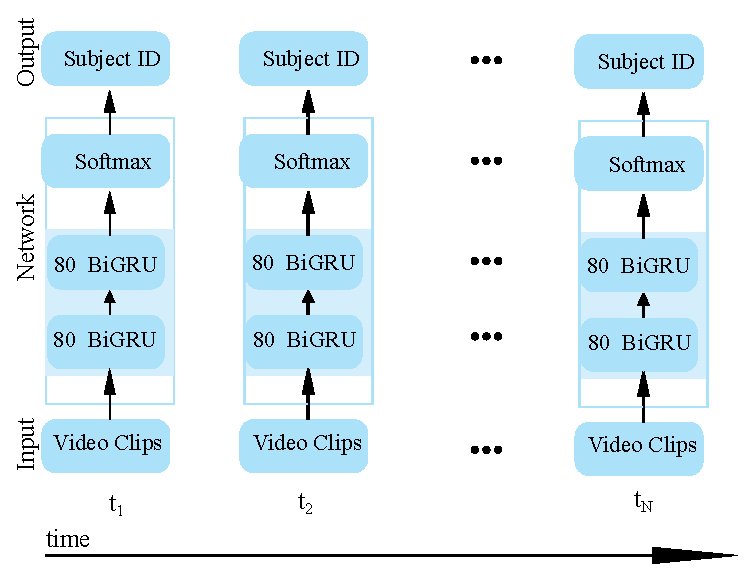
\includegraphics[width=0.7\textwidth ]{figures/output_prediction.eps}
	\caption[Output prediction scheme of our proposed network]{
		Output prediction scheme of the proposed network using majority voting scheme.
	}
	\label{fig:output_prediction}
\end{figure}

But, at the test time, we actually need the subject ID for the complete gait video. Therefore, we employed the \textit {majority voting scheme} algorithm to process this output to predict the subject ID. In this scheme, the subject that receives the highest number of votes over all timesteps in a  gait video is referred as the predicted class.

Let's consider, $\boldsymbol{s}$ is a vector IDs for $n$ number of subjects. For a particular timestep $t$, a gait video has input feature map $\boldsymbol X^t~\epsilon~\mathbb {R}^{28\times 50}$ and an n-dimensional output vector $\boldsymbol o^t$.

\begin{equation} \label{equ:timestep_sequence}
\begin{split}
\boldsymbol s^t &=  {[s_1, s_2, s_3, ....., s_{n}]}^{T}\\
\boldsymbol o^t &=  {[o_1, o_2, o_3, ....., o_{n}]}^{T}
\end{split}
\end{equation}

Here, $o_i^t = P(s_i | X^t)$ refers the probability of input feature map $\boldsymbol X^t$ belongs to class $s_i$. Now, we assign the output class $\mathbf{o}^t$ to the subject class $s_i$ which have maximum probabilities for the timestep $t$. As each of our gait videos is divided into a series of timestep sequence (see equation~\ref{equ:timestep_sequence}), using majority voting scheme we can calculate the subject ID. Following equations described the voting scheme:

\begin{equation}
\label{equ:predicted_class}
\begin{split}
s_t &=  \arg\max_{s_i}{\{o_i^t | 1 \leq i \leq n\}} \\
s &= {\arg\max}_{i\in(1, 2, ...,n)}{\sum_{t=1}^{N}s_i^N}
\end{split}
\end{equation}

Here, $ N $ is the total number of timesteps in which a gait is split and $ s $ is the final predicted class.  


\subsection{Training and Implementation Details}
The training of \gls{rnn}s allows us to learn the parameters from the sequence. We have employed Adam~\cite{Kingma_15} optimization algorithm with $\beta_1 = 0.9$ and $\beta_2 = 0.999$, which is known to work very well for training \gls{rnn}s. We tried several learning rates in our experiment and found out that the best initial learning rate is $(5$x$10^{-3})$. We also reduced the learning rate by a factor when it hit a plateau. Reducing the learning rate will allow the optimizer to get rid of the plateaus in the loss surface. Table~\ref{table:summary_tn} summarizes all the hyperparameters setting of our network.

\begin{table}
	\centering
	\caption{Training summary of our proposed temporal network. \label{table:summary_tn}}
	\begin{tabular*}{32pc}{@{\extracolsep{\fill}}ll@{}}
		\hline \noalign{\vspace{3pt}}
		\textbf{Hyperparameter} &\qquad \textbf{Value} \\ [3pt] \hline\noalign{\vspace{3pt}}
		Optimizer     			&\qquad Adam~\cite{Kingma_15} \\[3pt]
		Objective function  	&\qquad Fusion of softmax and center loss \\[3pt]
		Epochs        			&\qquad $ 450 $ \\ [3pt]
		Initial learning rate	&\qquad $5 \times 10^{-3}$  \\[3pt]
		Mini-batch size			&\qquad $ 256 $ \\
		\hline
	\end{tabular*}
\end{table}

The proposed network was trained with a batch size of $ 256 $ for $ 450 $ epochs. Our network showed some overfitting mostly due to the high learning capacity of the network over data. We addressed the overfitting problem by adding a \gls{bn} layer before and after the \gls{bigru} layer. We also tried to add a dropout~\cite{Srivastava_14} layer during training, but that did not help to reduce the overfitting problem. Moreover, it degraded the gait recognition performance. Hence, we skip it.

For the model computations, we entirely relied on GPU programming. In particular, our implementation was based on Keras~\cite{keras}, a GPU-capable deep-learning library written in Python. All the experiments were performed on a server machine with 56 cores, 512 GB RAM, and an Nvidia Tesla K40 graphic card with 12 GB memory running on Ubuntu server 18.04 LTS. Input video and image sequences were processed using Python and OpenCV library~\cite{opencv}.




\begin{figure}
	\centering
	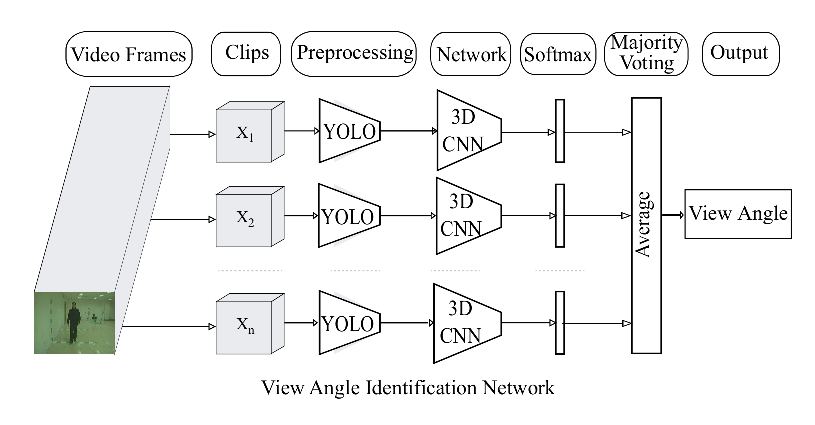
\includegraphics[width=0.94\textwidth]{figures/view_angle_identification.eps}
	\caption[Overview of our proposed view angle identification network scheme] 
	{Overview of our proposed view angle identification network scheme. \label{fig:view_angle_identification}
	}
\end{figure}

%-------------------------------------------------------------------------
\section{Multi-View Gait Recognition} \label{sec:multi_view_arch}
In this section, we will elaborate on the proposed two-stage network for multi-view gait recognition. 


\subsection{Preprocessing}
Firstly, to localize human walking direction in the gait videos, we employed YOLOv3, a state-of-the-art real-time object detection algorithm, proposed by Redmon \textit{et al.}~\cite{Redmon_18}. We then cropped each of the subject detected frame using the bounding box coordinates found from the YOLOv3 algorithm and resized them to $112\times112$ for our network input. Thereafter, we split each gait video into overlapping sequences of 16 consecutive frames within the training or test set. There is an overlap of 8 frames indicating that the samples were gathered using a 16 frame sliding window with a 50\% stride.


\subsection{3D Convolution for Video Classification}
Identifying walking direction from gait video is somewhat similar to the action recognition problem in computer vision. Recently, in action recognition, researchers have started to exploit 3D features in the video using the 3D-CNN model which extracts features from both spatial and temporal dimensions by performing 3D convolutions. Tran et.al.~\cite{Tran_15} proposed a 3D convolutional neural network, also known as C3D, which has been widely used for applications like video classification, action recognition, etc. Sports-1M~\cite{karpathy_14}, one of the largest benchmark datasets for video classification has been employed to train the network. The dataset contains $ 1.1$ million sports videos, where each video belongs to one of the 487 sports categories. 

\begin{table}
	\centering
	\caption{Training summary of our proposed 3D-CNN network.  \label{table:summary_3dcnn}}
	\begin{tabular*}{30pc}{@{\extracolsep{\fill}}ll@{}}
			\hline \noalign{\vspace{3pt}}
			\textbf{Hyperparameter} & \textbf{Value} \\ \hline\noalign{\vspace{3pt}}
			Optimizer  &Stochastic gradient descent (\gls{sgd})  \\ [3pt]
			Objective function  &Mean squared error (\gls{mse}) \\ [3pt]
			Epochs  &70  \\ [3pt]
			Initial learning rate & $1 \times 10^{-3}$ \\ [3pt]
			Mini-batch size	  &12  \\ [3pt]
			Momentum  &0.92 \\ [3pt]
			\hline
	\end{tabular*}
\end{table}

\begin{figure}[t]
	\centering {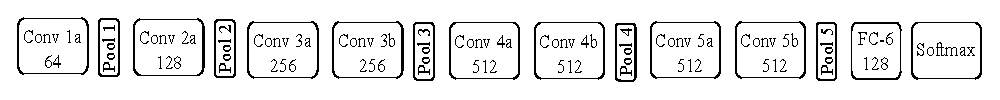
\includegraphics[width=\textwidth]{figures/3D_CNN.eps}}
	\caption[Fine tuning a pretrained C3D network for view angle identification.]
	{Fine tuning a pretrained C3D~\cite{Tran_15} network for view angle identification. \label{fig:3D_CNN}
	}
\end{figure}

\begin{figure}
	\centering {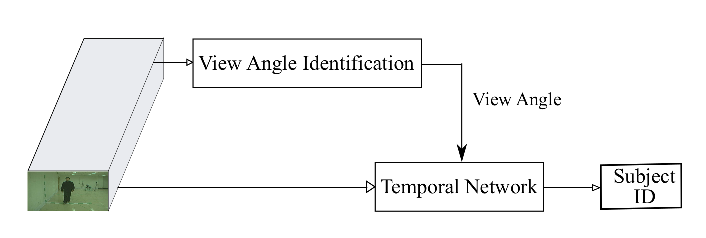
\includegraphics[width=0.8\textwidth]{figures/two-stage_network.eps}}
	\caption[Proposed two-stage network for multi-view gait recognition.]
	{Proposed two-stage network for multi-view gait recognition.\label{fig:two-stage_network}
	}
\end{figure}


\subsection{View Angle Identification}
Successful transfer learning within or across the different domains of interest leads to significant improvement in performance due to the amount of jointly learning representations in a shared feature space. In our work, we employed a pretrained C3D model and fine-tuned it for our 3D Convolutional network to determine the view angle of walking from gait. Figure~\ref{fig:3D_CNN} shows our proposed 3D convolutional network. 

C3D network is composed of 8 convolutional layers, 5 pooling layers, 2 fully-connected layers, followed by a softmax layer at the end. All the 3D convolution kernels are $3\times3\times3$ with stride 1 in both spatial and temporal dimensions. We removed the last 3 layer from the model and then added a fully connected layer of 128 neurons and a dropout~\cite{Srivastava_14} layer of 0.5 to avoid overfitting. Finally, a softmax layer of 11 neurons has been added to classify any given videos into 11 different viewing angles. 

The proposed method for our view angle identification is illustrated in Figure~\ref{fig:view_angle_identification}. The input of the network was a clip of 16 consecutive frames which was preprocessed and resized to $112\times112$ to feed into a  3D-CNN network. We used the {\textit {majority voting scheme}} to process the output to predict the view angle similar to section~\ref{subsec_post_process}, i.e. the angle that receives the highest number of votes over all clips are referred as the predicted angle of the gait.



\subsection{Two-Stage Network}
Figure~\ref{fig:two-stage_network} illustrates the proposed two-stage network for multi-view gait recognition. Firstly, a view angle identification network was employed to identify the subject's walking direction. In this study, a 3D convolutional network was trained to estimate the walking direction of the subject by extracting spatio-temporal features from the gait video. Henceforth, we will perform subject identification using the proposed temporal network that was trained on that view angle.


\subsubsection{Training Details}
We employed the CASIA B gait dataset~\cite{Yu_06} to train our model. We trained the network using 4 normal walking sequences of 100 subjects in the gallery set of CASIA B as described in Table~\ref{table:caisab_setup}. Our network was trained with a 12 batch size with an initial learning rate ${10^{-3}}$ for 70 epochs. Table~\ref{table:summary_3dcnn} summarizes all of the hyperparameters settings of our proposed network.

